\documentclass[12pt,a4paper]{report}
\usepackage[brazilian, english]{babel}
\usepackage[utf8]{inputenc}
\usepackage[T1]{fontenc}
\usepackage{amsmath,amsthm,amsfonts,amssymb,textcomp}
%\usepackage{latexsym}
\usepackage{graphicx}
\graphicspath{{figuras}}
\usepackage{subfigure}
\usepackage{float}
\usepackage{longtable}
\usepackage{color}
\usepackage{epstopdf}
\usepackage{pdflscape}
\usepackage[breaklinks=true]{hyperref}
\usepackage[comma,authoryear]{natbib}
\usepackage[nonumberlist]{glossaries}
\usepackage{arydshln}
\usepackage{footnote}
\usepackage{longtable}
\usepackage[small,bf,singlelinecheck=off]{caption}
\usepackage[left=3cm,right=2cm,top=3cm,bottom=2cm]{geometry}
%\usepackage[alf]{abntcite}

%%% newcommand %%%%%%%%%%%%%%%%%
\newcommand{\PE}{Perkin-Elmer }
\newcommand{\BC}{Boller \& Chivens }

\newcommand{\degr}{\ensuremath{^{\circ}}}%                    % degree symbol:  °
\newcommand{\arcmin}{\ensuremath{^{\prime}}}%                    % degree symbol:  °
\newcommand{\arcsec}{\ensuremath{^{\prime\prime}}}%                    % degree symbol:  °
\newcommand{\fs}{\mbox{\ensuremath{.\!\!^s}}}
\newcommand{\farcm}{\mbox{\ensuremath{.\mkern-4mu^\prime}}}%    % fractional arcminute symbol: 0.'0
\newcommand{\farcs}{\mbox{\ensuremath{.\!\!^{\prime\prime}}}}%  % fractional arcsecond symbol: 0.''0
\newcommand{\fdg}{\mbox{\ensuremath{.\!\!^\circ}}}%             % fractional degree symbol:     0.°0



%\makeglossaries

\makeatletter
\renewcommand\chapter{\thispagestyle{plain}
                \global\@topnum\z@
                \@afterindentfalse
                \secdef\@chapter\@schapter}
\makeatother


\makeatletter
\renewcommand{\@makechapterhead}[1]{%
\vspace*{50 pt}%
{\setlength{\parindent}{0pt} \raggedright \normalfont
\bfseries\Huge\thechapter.\ #1
\par\nobreak\vspace{40 pt}}}
\makeatother

%\newglossaryentry{Offset}{name={Offset}, description={Diferença entre a posição obtida pela redução da observação e a posição dada pela efeméride}}
\newglossaryentry{OPD}{name={OPD}, description={Observatório do Pico dos Dias - Brasópolis, MG}}
\newglossaryentry{LNA}{name={LNA}, description={Laboratório Nacional de Astrofísica - Itajubá, MG}}
\newglossaryentry{OHP}{name={OHP}, description={Observatoire Haute Provence - Saint-Michel-l'Observatoire, França}}
\newglossaryentry{RA}{name={RA}, description={Sigla para Ascensão Reta ($ \alpha $)}}
\newglossaryentry{DEC}{name={DEC}, description={Sigla para Declinação ($ \delta $)}}
\newglossaryentry{Anomalia Verdadeira}{name={Anomalia Verdadeira}, description={Ângulo formado entre o Periastro e a posição instantânea do objeto na órbita centrado no planeta e contada na direção do movimento orbital}}
\author{Altair Ramos Gomes Júnior}
\title{Astrometry of the Neptune-Triton System}
\begin{document}

\maketitle

\pagestyle{headings}

\section*{Chromatic Refraction}

Since the colors of Neptune and Triton are different, it is expected that their positions have influence of chromatic refraction with different intensities. The apparent position of Neptune, which is more blue than Triton, would be more shifted towards the zenith than the Triton's position.

To test the effects of chromatic refraction I looked for nights with many observations distributed over the night. I selected two of them (August 22, 2004 and September 25, 2011) with more than 4 hours between the first and last observations. In the night of 2004 it was used a filter called "Dark" which we suppose it means no filter, however we are no sure so I classified it as unknown. In the night of 2011 it was used a I filter.

In Fig \ref{Fig:refraction} it is plotted the difference in the positions of Triton and Neptune compared to the difference of their ephemeris in RA and DEC for both nights.

\begin{figure}[h]
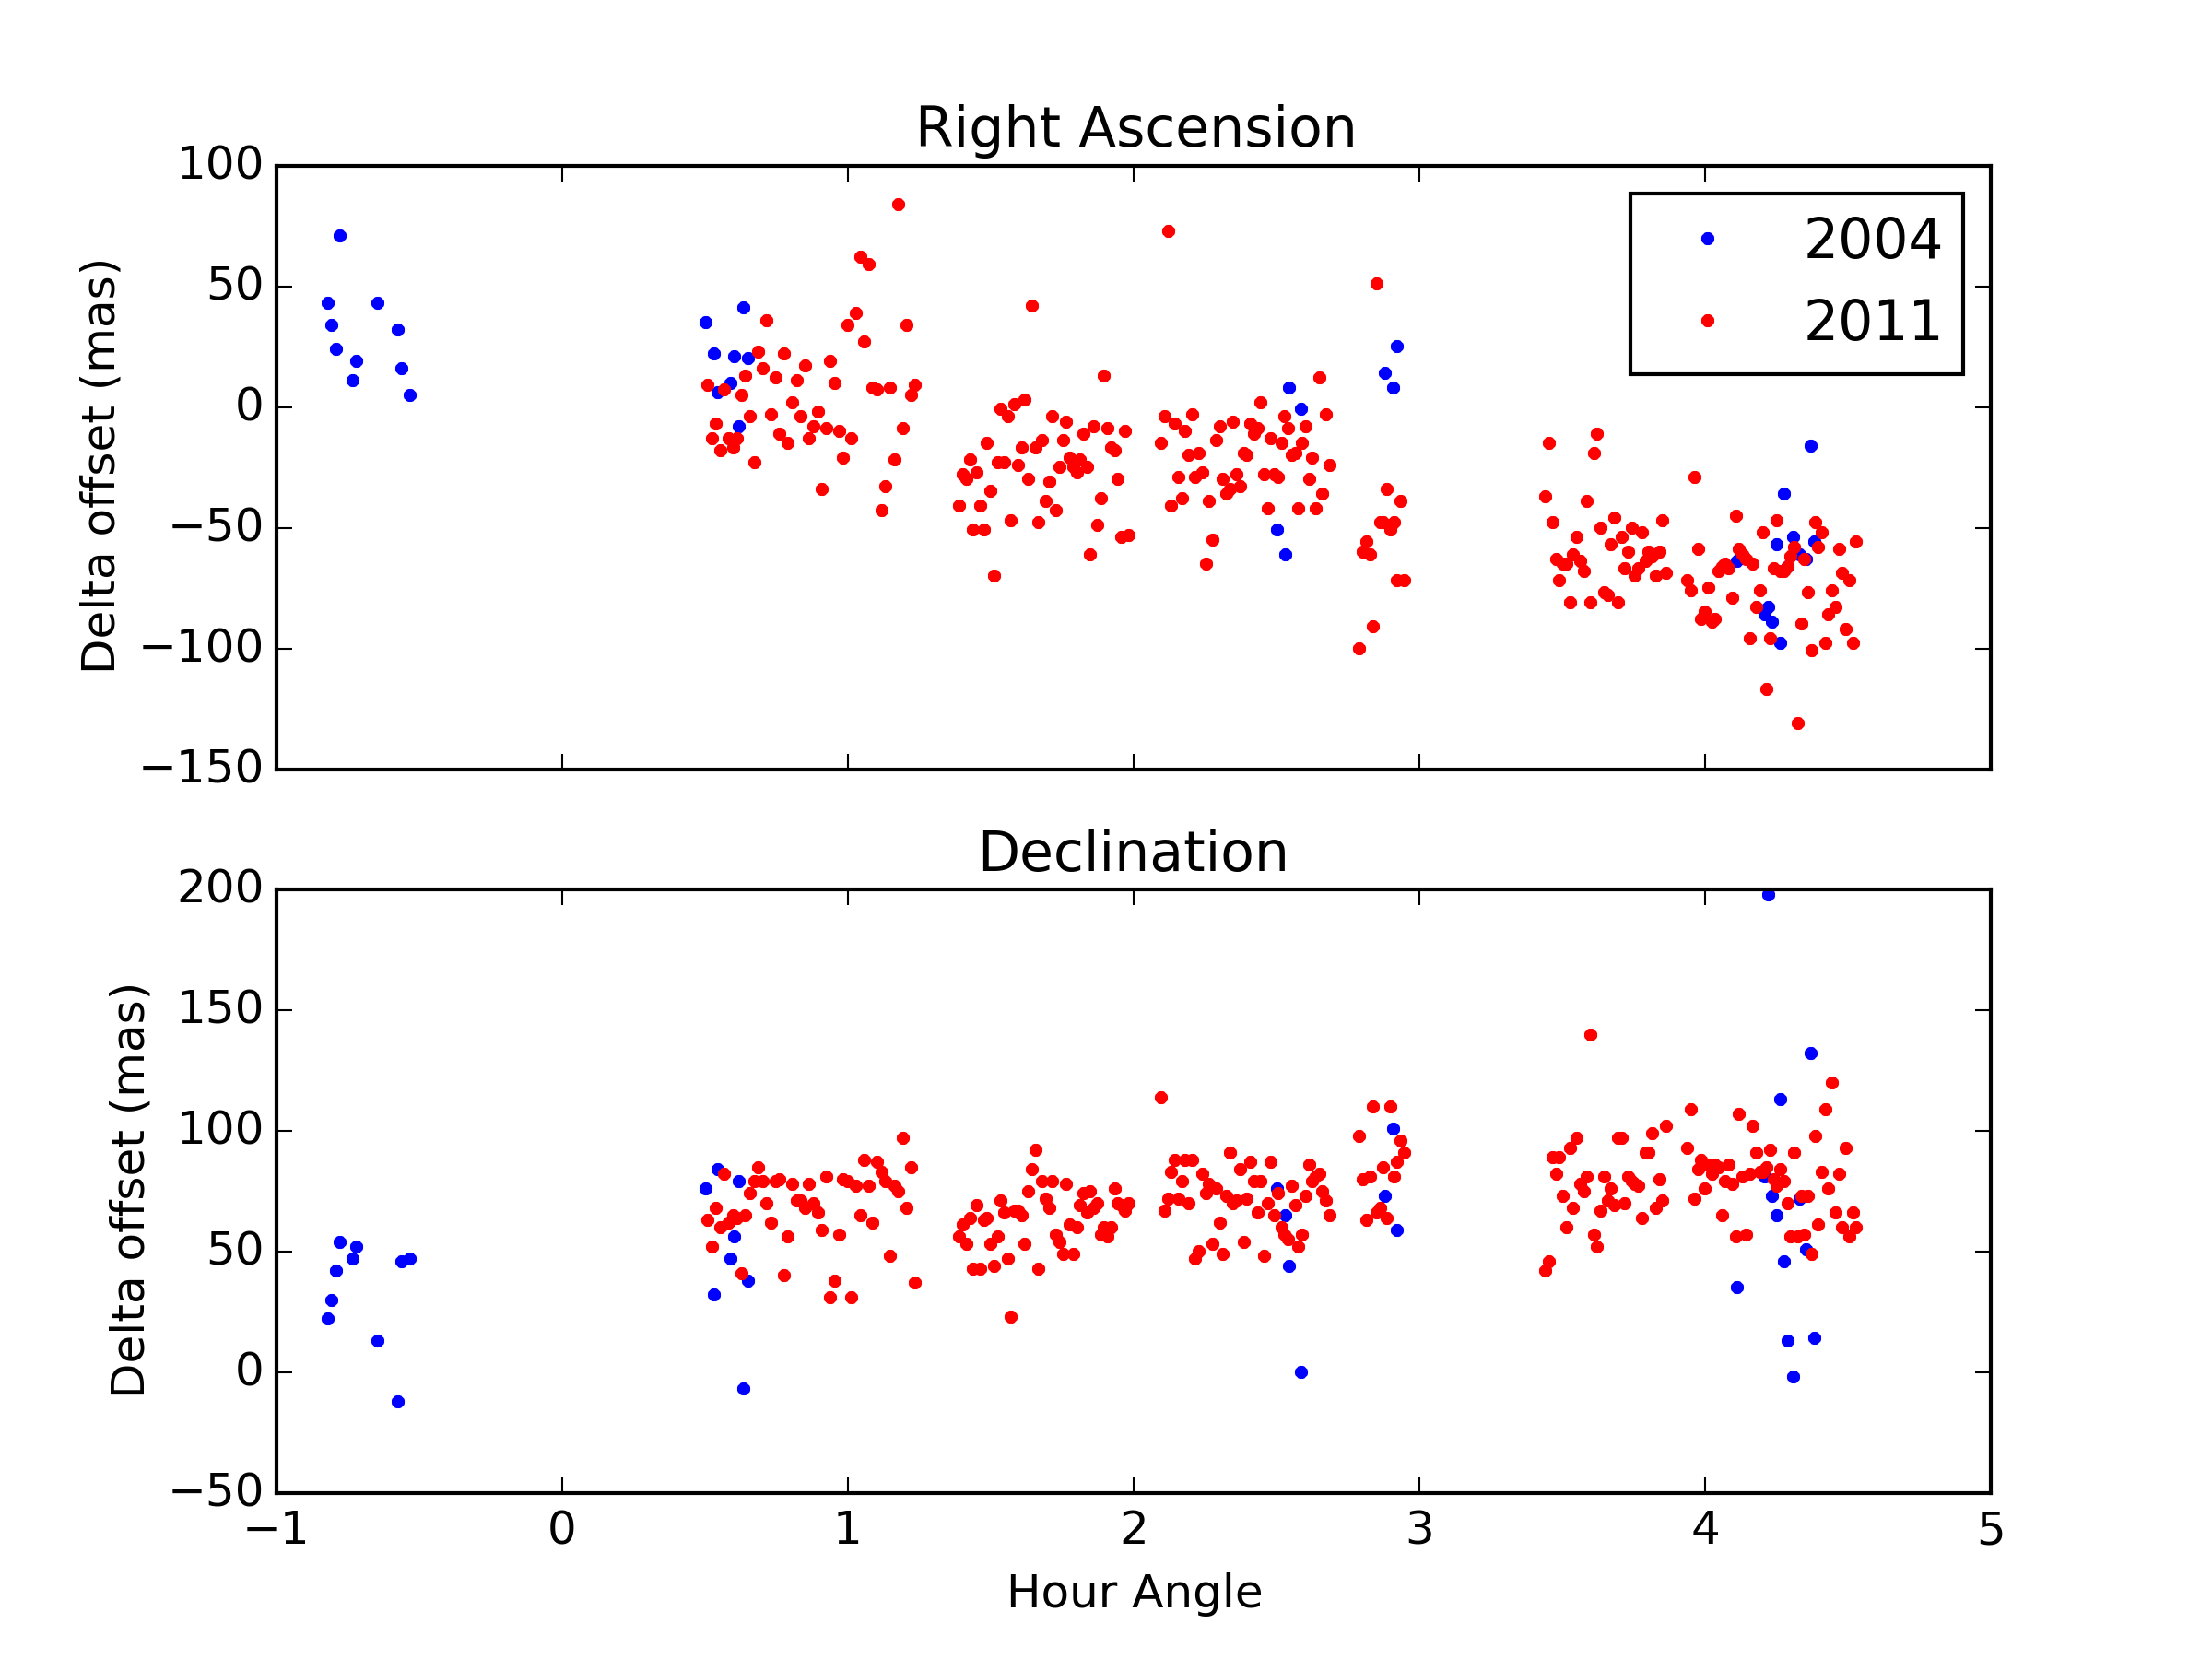
\includegraphics[width=16.0cm]{plot_hour_gr1.png} 
\caption{Distribution of the difference of offsets in the sense Triton - Neptune for the nights August 22, 2004 and September 25, 2011.}
\label{Fig:refraction}
\end{figure}

Teoretically, the difference in the positions of the objects in the sense Triton - Neptune compared to the difference in the ephemeris over a night would cause the following effects.

\begin{itemize}
\item RA: the difference in the offsets would be positives in the East side of the sky, negative in the West side and zero in the culmination, with the assumption that only chromatic refraction affects the offsets.
\item DEC: the difference in the offsets in the culmination would be positive (Neptune is in the North side in both nights for the site). Farther from the culmination the difference in the offsets would be more positive.
\end{itemize}

Fig \ref{Fig:refraction} clearly shows that that the chromatic refraction is affecting the offsets confirming our expectation.


\begin{table*}[h]
\centering
\caption{Difference in the offsets of Triton-Neptune of the nights used as tests of chromatic refraction with sigma-clipping procedure}
\label{Tab:dados}
\begin{tabular}{|c|c|c|c|c|c|c|}
\hline 
Night & N & $\mu$ RA & $\mu$ DEC & $\sigma$ RA & $\sigma$ DEC & Ncat\\
\hline
2004-08-22 & 29 & 2 & 45 & 34 & 28 & 13 \\ 
2011-09-25 & 106 & -20 & 67 & 11 & 11 & 17\\
\hline 
\end{tabular}
\\N: Number of positions after sigma-clipping procedure. Ncat is the number UCAC4 stars used in the reductions.
\end{table*}





\end{document}
